\documentclass[../basicOrbitalDynamics.tex]{subfiles}
\graphicspath{{\subfix{../images/}}}
\begin{document}

\bigskip\bigskip
\subsection{Inclination Change}

In Section \ref{sec:Mn Manuever}, maneuvers were done at a constant angle to the velocity vector. However, it is more efficient to transfer to the desired orbit directly by finding the vector difference between the old velocity and the desired velocity. To maximize the effect of such a manuever, it should be done at either the ascending or descending node (such that $\Delta j=\Delta i$).

\begin{figure}[H]
    \centering
    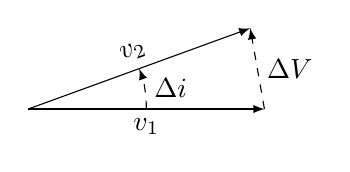
\begin{tikzpicture}[>=latex]
        \def\vel{3}
        \def\dPhi{20}
        \def\arcRad{1.5}

        \draw[->] (0,0) -- +(\dPhi:\vel) node[midway,above,sloped] {$v_2$};
        \draw[->] (0,0) -- +(\vel,0) node[midway,below] {$v_1$};
        \draw[dashed, ->] (\vel,0) -- (\dPhi:\vel) node[midway,right] {$\Delta V$};
        \draw[dashed, ->] (\arcRad,0) arc (0:\dPhi:\arcRad) node[midway, right] {$\Delta i$};
    \end{tikzpicture}
    \caption{Inclination change velocity}\label{fig:dV Triangle Inclination Chage}
\end{figure}

Because the only effect of this maneuver is to change the direction of velocity, $\Delta V$ is the magnitude of the vector difference in the old velocity and the new velocity. Note that, throughout this maneuver, the magnitude of velocity will first decrease and then increase, so there is no net effect on the shape of the orbit in its own plane.

\begin{align*}
    \Delta V &= |\vv{v}_2-\vv{v}_1| \\
    &= |(v\cos(\Delta i)\hat{m}_v+v\sin(\Delta i)\hat{m}_n)-(v\hat{m}_v)| \\
    &= |v(\cos(\Delta i)-1)\hat{m}_v+v\sin(\Delta i)\hat{m}_n| \\
    &= \sqrt{(v(\cos(\Delta i)-1))^2+(v\sin(\Delta i))^2} \\
    &= \sqrt{v^2(\cos(\Delta i)-1)^2+v^2\sin^2(\Delta i)} \\
    &= v\sqrt{(\cos(\Delta i)-1)^2+\sin^2(\Delta i)} \\
    &= v\sqrt{\cos^2(\Delta i)+1-2\cos(\Delta i)+\sin^2(\Delta i)} \\
    &= v\sqrt{(\cos^2(\Delta i)+\cos^2(\Delta i))+1-2\cos(\Delta i)} \\
    &= v\sqrt{2-2\cos(\Delta i)} \\
    &= v\sqrt{2(1-\cos(\Delta i))} \\
    &= v\sqrt{2\left(1-\cos\left(2\frac{\Delta i}{2}\right)\right)} \\
    &= v\sqrt{4\left(\frac{1-\cos\left(2\frac{\Delta i}{2}\right)}{2}\right)} \\
    &= v\sqrt{4\sin^2\left(\frac{\Delta i}{2}\right)} \\
\end{align*}

This gives us the $\Delta V$ required for an inclination change maneuver
\begin{equation}
    \Delta V= 2\sin\left(\frac{\Delta i}{2}\right)
\end{equation}

This shows the minimum required $\Delta V$ for an orbital inclination change. If the inclination change occurs at any point other than the ascending or descending node, it will require a greater $\Delta V$ and will also have the effect of chaning the longitude of ascending node $\Omega$ (and therefore moving the ascending and descending nodes). In-plane maneuvers will change neither the inclination nor the longitude of ascending node.

\bigskip\bigskip
\subsection{Hohmann Transfer}\label{sec:Hohmann Transfer}

A Hohmann Transfer is a transfer between two circular orbits from radius $r_1$ to radius $r_2$. The transfer is done via an elliptical orbit, and takes two burns. The first burn puts the orbit into an elliptical orbit in which the periapsis is the lower orbit, and the apoapsis is the higher orbit. The second burn transfers from the elliptic orbit into the final circular orbit.

\begin{figure}[H]
    \centering
    \def\Rone{0.75}
    \def\Rtwo{2.5}
    \def\transSMA{\fpeval{(\Rone+\Rtwo)/2}}
    \def\ctrX{\fpeval{\Rone-\transSMA}}
    \def\trE{\fpeval{\Rtwo/\transSMA - 1}}
    \def\transSmA{\fpeval{\transSMA*sqrt(1-(\trE)^2)}}
    \def\dV{1.25}
    \definecolor{purp}{rgb}{.8,0,.8}
    \begin{tikzpicture}[>=latex]
        \draw[thin, dotted, blue] (0,0) ellipse ({\Rone} and {\Rone});
        \draw[blue, thick,>-] (-\Rone,0) arc (180:360:{\Rone} and {\Rone}) node[right] {$r_1$};


        \draw[thin, dotted, purp] (\ctrX,0) ellipse ({\transSMA} and {\transSmA});
        \draw[purp, thick] (\Rone,0) arc (0:180:{\transSMA} and {\transSmA});

        \draw[thin, dotted,red] (0,0) ellipse ({\Rtwo} and {\Rtwo});
        \draw[red, thick,->] (-\Rtwo,0) arc (180:360:{\Rtwo} and {\Rtwo}) node[right] {$r_2$};;

        \filldraw[lightgray] (0,0) circle (2pt);

        \draw[->] (\Rone,0)--+(0,\dV) node[above] {$\Delta v_1$};
        \draw[->] (-\Rtwo,0)--+(0,-\dV) node[below] {$\Delta v_2$};

    \end{tikzpicture}
    \begin{tikzpicture}[>=latex]
        \draw[->] (\Rone,0)--+(0,-\dV) node[below] {$\Delta v_1$};
        \draw[->] (-\Rtwo,0)--+(0,\dV) node[above] {$\Delta v_2$};

        \draw[thin, dotted, red] (0,0) ellipse ({\Rone} and {\Rone});
        \draw[red, thick,->] (\Rone,0) arc (0:180:{\Rone} and {\Rone}) node[left] {$r_2$};


        \draw[thin, dotted, purp] (\ctrX,0) ellipse ({\transSMA} and {\transSmA});
        \draw[purp, thick] (-\Rtwo,0) arc (180:360:{\transSMA} and {\transSmA});

        \draw[thin, dotted,blue] (0,0) ellipse ({\Rtwo} and {\Rtwo});
        \draw[blue, thick,>-] (\Rtwo,0) arc (0:180:{\Rtwo} and {\Rtwo}) node[left] {$r_1$};;

        \filldraw[lightgray] (0,0) circle (2pt);

    \end{tikzpicture}
    \caption{A Hohmann Transfer from a low orbit to a high orbit (left) and from a high orbit to a lower one (right)}\label{fig:Hohmann Transfer}
\end{figure}

Because both burns are along the velocity vector, $\Delta V=\Delta v_1+\Delta v_2$. $a_1=r_1=\st{r}{pe,tr}$ will refer to the semi-major axis of the smaller orbit, with $a_2=r_2=\st{r}{ap,tr}$ being the semi-major axis of the larger orbit. The semi-major axis of the transfer orbit is $\st{a}{tr}=\frac{1}{2}(r_1+r_2)$. $v_1$ and $v_2$ refer to the circular orbit velocities in the original and new orbit. The below calculations assume a transfer from a low orbit into a higher one.

\begin{align*}
    \Delta V &= \Delta v_1+\Delta v_2\\
    &= |\st{v}{pe,tr}-v_1|+|v_2-\st{v}{ap,tr}|\\
    &= \left|\sqrt{\frac{2\mu}{\st{r}{pe,tr}}-\frac{\mu}{\st{a}{tr}}}-\sqrt{\frac{2\mu}{r_1}-\frac{\mu}{a_1}}\right|+\left|\sqrt{\frac{2\mu}{\st{r}{ap,tr}}-\frac{\mu}{a_2}}-\sqrt{\frac{2\mu}{r_2}-\frac{\mu}{\st{a}{tr}}}\right| \\
    &= \left|\sqrt{\frac{2\mu}{r_1}-\frac{\mu}{\frac{1}{2}(r_1+r_2)}}-\sqrt{\frac{2\mu}{r_1}-\frac{\mu}{r_1}}\right|+\left|\sqrt{\frac{2\mu}{r_2}-\frac{\mu}{r_2}}-\sqrt{\frac{2\mu}{r_2}-\frac{\mu}{\frac{1}{2}(r_1+r_2)}}\right|\\
    &= \left|\sqrt{\frac{2\mu}{r_1}-\frac{\mu}{\frac{1}{2}(r_1+r_2)}}-\sqrt{\frac{\mu}{r_1}}\right|+\left|\sqrt{\frac{\mu}{r_2}}-\sqrt{\frac{2\mu}{r_2}-\frac{\mu}{\frac{1}{2}(r_1+r_2)}}\right|\\
    &= \left|\sqrt{\frac{2\mu}{r_1}-\frac{\mu}{\frac{1}{2}(r_1+r_2)}}-\sqrt{\frac{\mu}{r_1}}\right|+\left|\sqrt{\frac{\mu}{r_2}}-\sqrt{\frac{2\mu}{r_2}-\frac{\mu}{\frac{1}{2}(r_1+r_2)}}\right|\\
    &= \left|\sqrt{\frac{2\mu}{r_1}-\frac{2\mu}{r_1+r_2}}-\sqrt{\frac{\mu}{r_1}}\right|+\left|\sqrt{\frac{\mu}{r_2}}-\sqrt{\frac{2\mu}{r_2}-\frac{2\mu}{r_1+r_2}}\right|\\
    &= \left|\sqrt{\frac{2\mu(r_1+r_2)}{r_1(r_1+r_2)}-\frac{2\mu{}r_1}{r_1(r_1+r_2)}}-\sqrt{\frac{\mu}{r_1}}\right|+\left|\sqrt{\frac{\mu}{r_2}}-\sqrt{\frac{2\mu(r_1+r_2)}{r_2(r_1+r_2)}-\frac{2\mu{}r_2}{r_2(r_1+r_2)}}\right|\\
    &= \left|\sqrt{\frac{2\mu(r_1+r_2)-2\mu{}r_1}{r_1(r_1+r_2)}}-\sqrt{\frac{\mu}{r_1}}\right|+\left|\sqrt{\frac{\mu}{r_2}}-\sqrt{\frac{2\mu(r_1+r_2)-2\mu{}r_1}{r_2(r_1+r_2)}}\right|\\
    &= \left|\sqrt{\frac{2\mu{}r_2}{r_1(r_1+r_2)}}-\sqrt{\frac{\mu}{r_1}}\right|+\left|\sqrt{\frac{\mu}{r_2}}-\sqrt{\frac{2\mu{}r_1}{r_2(r_1+r_2)}}\right|\\
\end{align*}

Note that both absolute value terms will have the same sign; they will either both be positive, or both be negative. Therefore, they can be absorbed under the same absolute value.

\begin{equation}\label{Hohmann Delta V}
    \Delta V = \left|\sqrt{\frac{2\mu{}r_2}{r_1(r_1+r_2)}}+\sqrt{\frac{\mu}{r_2}}-\sqrt{\frac{2\mu{}r_1}{r_2(r_1+r_2)}}-\sqrt{\frac{\mu}{r_1}}\right|\\
\end{equation}

Note that this equation is the same if $r_1$ and $r_2$ are swapped. Therefore, $\Delta V$ does not depend on the direction of the transfer; a transfer between the same two circular orbits will have the same $\Delta V$ regardless of whether the transfer is from a high orbit to a low one, or from the low orbit to a the higher one.

The time for this transfer is simply half the period of the transfer orbit, which can be calculated using Equation \eqref{Period Geometric}.

\begin{align*}
    t &= \frac{\st{T}{tr}}{2} \\
 &= \frac{1}{2}\sqrt{\frac{4\pi^2 \st{a}{tr}^3}{\mu}} \\
 &= \pi\sqrt{\frac{\st{a}{tr}^3}{\mu}} \\
 &= \pi\sqrt{\frac{\left(\frac{1}{2}(r_1+r_2)\right)^3}{\mu}} \\
\end{align*}

Giving us a total transfer time of

\begin{equation}\label{Hohmann time}
    \st{T}{tr}=\pi\sqrt{\frac{(r_1+r_2)^3}{8\mu}}
\end{equation}

\subsubsection{\texorpdfstring{$\Delta V$}{DeltaV} Analysis for Hohmann Transfers}\label{sec:DeltaV analysis for Hohmann}

Equation \eqref{Hohmann Delta V} will be written with $\st{r}{high}=r_2$ and $\st{r}{low}=r_1$. A parameter $\alpha$ is defined as $\alpha=\st{r}{high}/\st{r}{low}$, allowing $\Delta V$ to be made a function of $\alpha$.

\begin{align*}
    \Delta V &= \left|\sqrt{\frac{2\mu{}\st{r}{high}}{\st{r}{low}(\st{r}{low}+\st{r}{high})}}+\sqrt{\frac{\mu}{\st{r}{high}}}-\sqrt{\frac{2\mu{}\st{r}{low}}{\st{r}{high}(\st{r}{low}+\st{r}{high})}}-\sqrt{\frac{\mu}{\st{r}{low}}}\right|\\
    &= \left|\sqrt{\frac{2\mu{}(\st{r}{low}\alpha)}{\st{r}{low}(\st{r}{low}+(\st{r}{low}\alpha))}}+\sqrt{\frac{\mu}{\st{r}{low}\alpha}}-\sqrt{\frac{2\mu{}\st{r}{low}}{(\st{r}{low}\alpha)(\st{r}{low}+(\st{r}{low}\alpha))}}-\sqrt{\frac{\mu}{\st{r}{low}}}\right| \\
    &= \left|\sqrt{\frac{2\mu\alpha}{\st{r}{low}+\st{r}{low}\alpha}}+\sqrt{\frac{\mu}{\st{r}{low}\alpha}}-\sqrt{\frac{2\mu}{\alpha(\st{r}{low}+\st{r}{low}\alpha)}}-\sqrt{\frac{\mu}{\st{r}{low}}}\right| \\
    &= \left|\sqrt{\frac{2\mu\alpha}{\st{r}{low}(1+\alpha)}}+\sqrt{\frac{\mu}{\st{r}{low}\alpha}}-\sqrt{\frac{2\mu}{\st{r}{low}\alpha(1+\alpha)}}-\sqrt{\frac{\mu}{\st{r}{low}}}\right| \\
    &= \left|\sqrt{\frac{2\mu}{\st{r}{low}}}\sqrt{\frac{\alpha}{1+\alpha}}+\sqrt{\frac{\mu}{\st{r}{low}}}\sqrt{\frac{1}{\alpha}}-\sqrt{\frac{2\mu}{\st{r}{low}}}\sqrt{\frac{1}{\alpha(1+\alpha)}}-\sqrt{\frac{\mu}{\st{r}{low}}}\right| \\
    &= \left|\sqrt{\frac{\mu}{\st{r}{low}}}\sqrt{\frac{2\alpha}{1+\alpha}}+\sqrt{\frac{\mu}{\st{r}{low}}}\sqrt{\frac{1}{\alpha}}-\sqrt{\frac{\mu}{\st{r}{low}}}\sqrt{\frac{2}{\alpha(1+\alpha)}}-\sqrt{\frac{\mu}{\st{r}{low}}}\right| \\
    &= \sqrt{\frac{\mu}{\st{r}{low}}}\left|\sqrt{\frac{2\alpha}{1+\alpha}}+\sqrt{\frac{1}{\alpha}}-\sqrt{\frac{2}{\alpha(1+\alpha)}}-1\right| \\
\end{align*}

Because $\alpha>1$, the absolute value can vanish as its argument will always be positive.

\begin{equation}\label{Delta V in terms of Alpha Hohmann}
    \Delta V(\alpha, \st{r}{low}) = \sqrt{\frac{\mu}{\st{r}{low}}}\left(\sqrt{\frac{2\alpha}{1+\alpha}}+\sqrt{\frac{1}{\alpha}}-\sqrt{\frac{2}{\alpha(1+\alpha)}}-1\right)\\
\end{equation}

Notice that the coefficient $\sqrt{\mu/\st{r}{low}}$ is the circular velocity at the low orbit.

By plotting $\Delta V$ against $\alpha$, a trend can be found. From Equation \eqref{Delta V in terms of Alpha Hohmann}, the exact value of $\st{r}{low}$ only scales the plot of $\Delta V(\alpha)$ but does not effect its shape.
\begin{figure}[H]
    \centering
    \def\rootMuOverR{5}
    \begin{tikzpicture}[>=latex]
        \draw[->] (0,0)--+(10,0) node[midway, below] {$\alpha=\st{r}{high}/\st{r}{low}$};
        \draw[->] (0,0)--+(0,3) node[midway, left] {$\Delta V$};

        \draw[domain=1:10, smooth, ->] plot (\x, {\rootMuOverR*(sqrt(2*\x/(1+\x))+sqrt(1/\x)-sqrt(2/(\x*(\x+1)))-1)});
        %\draw[domain=0.4:1, smooth, <-] plot (\x, {-5*(sqrt(2*\x/(\R*(1+\x)))+sqrt(1/(\x*\R))-sqrt(2/(\R*\x*(\x+1)))-sqrt(1/\R))});
        \draw[gray , dashed] (1,0) -- +(0,3) node[midway, sloped, above] {$\alpha=1$};

    \end{tikzpicture}
    \caption{Plot of $\Delta V$ vs $\alpha$ with $\st{r}{low}$ held constant}\label{fig:Hohmann Delta V r1 const}
\end{figure}

It is important to note that the apparent behavior of constant increase is not the true behavior of this function. The function exhibits a maximum at $\alpha\approx15.58172$ (the work for this is not shown, as differentiation of \eqref{Delta V in terms of Alpha Hohmann} is rather tedious, and the roots of the derivative cannot be found analytically), and then exhibits the following limiting behavior
$$\lim_{\alpha\rightarrow\infty}\Delta V(\alpha, \st{r}{low})=(\sqrt{2}-1)\sqrt{\frac{\mu}{\st{r}{low}}}$$

%TODO: HOLD rHIGH constant!
If instead $\alpha$ is held constant, then the relationship between $\st{r}{low}$ and $\Delta V$ can be explored. As can be seen in Equation \eqref{Delta V in terms of Alpha Hohmann}, the value of $\alpha$ does not impact the shape of the plot of $\Delta V(\st{r}{low})$, but instead scales it. The general behavior of $\Delta V(\st{r}{low})$ follows $\st{r}{low}^{-0.5}$.

\begin{figure}[H]
    \centering
    \def\multBy{1.25}
    \begin{tikzpicture}[>=latex]
        \draw[->] (0,0)--+(10,0) node[midway, below] {$\st{r}{low}$};
        \draw[->] (0,0)--+(0,3) node[midway, left] {$\Delta V$};

        \draw[domain=1:10, smooth, ->] plot (\x, {\multBy*sqrt(1/\x)});
        \draw[domain=0.2:1, smooth, <-] plot (\x, {\multBy*sqrt(1/\x)});

    \end{tikzpicture}
    \caption{Plot of $\Delta V$ vs $\st{r}{low}$ with $\alpha$ held constant}\label{fig:Hohmann Delta V alpha const}
\end{figure}

The $\Delta V$ for a Hohmann Transfer can also be plotted as a heatmap, with one axis being origin orbit radius and the other being destination orbit radius.

\begin{figure}[H]
    \centering
    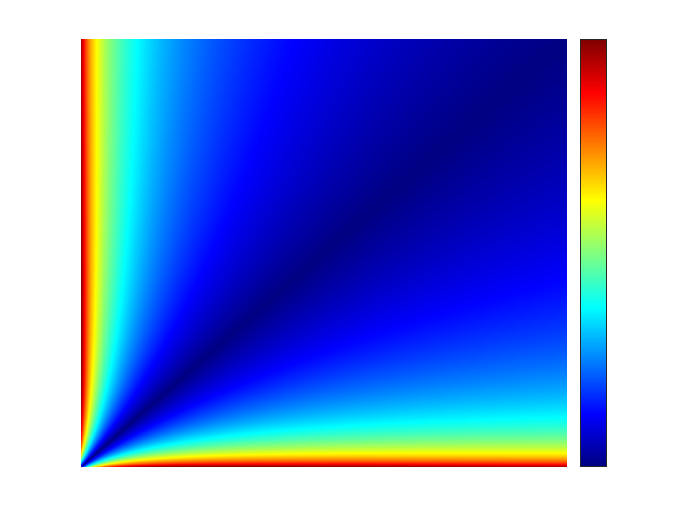
\includegraphics[scale=0.5]{DeltaVHeatmap.png}
    \caption{$\Delta V$ required for a Hohmann transfer between two orbits (created with MATLAB)}\label{fig:Delta V Heatmap}
\end{figure}

In the above figure, $\Delta V$ is represented by the colors, while the axes correspond to the destination and origin orbit radii. It can be seen that the highest $\Delta V$ expenditure occurs when one orbit is very low, while the other is very high.
\bigskip\bigskip
\subsection{Expedited Transfer}

It may at times be the case that the Hohmann Transfer is simply too slow for some applications. If the transfer is from a low orbit to a higher one, then the apoapsis of the transfer orbit can simply be raised higher than the destination orbit. Calculating the $\Delta V$ of such a transfer is elementary, as it requires only application of Equation \eqref{Vis-Viva Equation}. Using Equation \eqref{Time since periapsis}, the transfer time can be evaluated.

\bigskip\bigskip
\subsection{Bi-Elliptic Transfer}

A bi-elliptic transfer is another means of transferring from one circular orbit to another. While a Hohmann transfer takes a spacecraft from one circular orbit to another via a singular transfer orbit, the bi-elliptic transfer utilizes a series of two transfer orbits. First, the spacecraft is put into an orbit much higher than either the source or destination orbit. Then, at the apoapsis of the high transfer orbit, the periapsis is brought to the new orbit. Bi-elliptic transfers take advantage of the efficiencies of apsidal changes at high altitudes, and as such the transfer orbit will \textit{always} be higher than the origin or destination orbits.

\begin{figure}[H]
    \centering
    \def\Rone{0.75}
    \def\Rtwo{1.25}
    \def\trAP{4}
    \def\trSMAa{\fpeval{0.5*(\Rone+\trAP)}}
    \def\trSMAb{\fpeval{0.5*(\Rtwo+\trAP)}}
    \def\trEa{\fpeval{(\trAP/\trSMAa) - 1}}
    \def\trEb{\fpeval{(\trAP/\trSMAb) - 1}}
    \def\ctrXa{\fpeval{\Rone-\trSMAa}}
    \def\ctrXb{\fpeval{\Rtwo-\trSMAb}}
    \def\trSmAa{\fpeval{\trSMAa*sqrt(1-(\trEa)^2)}}
    \def\trSmAb{\fpeval{\trSMAb*sqrt(1-(\trEb)^2)}}
    \def\dV{1.25}
    \definecolor{purp}{rgb}{.8,0,.8}
    \definecolor{rurp}{rgb}{.8,0,.4}
    \begin{tikzpicture}[>=latex]
        \draw[thin, dotted, blue] (0,0) ellipse ({\Rone} and {\Rone});
        \draw[blue, thick,>-] (-\Rone,0) arc (180:360:{\Rone} and {\Rone}) node[midway, above] {$r_1$};

        \draw[thin, dotted, purp] (\ctrXa,0) ellipse ({\trSMAa} and {\trSmAa});
        \draw[purp, thick] (\Rone,0) arc (0:180:{\trSMAa} and {\trSmAa}) node[rurp, left] {$r_t$};

        \draw[thin, dotted, red] (\ctrXb,0) ellipse ({\trSMAb} and {\trSmAb});
        \draw[red, thick] (-\trAP,0) arc (180:360:{\trSMAb} and {\trSmAb});

        \draw[thin, dotted,orange] (0,0) ellipse ({\Rtwo} and {\Rtwo});
        \draw[orange, thick,->] (\Rtwo,0) arc (0:180:{\Rtwo} and {\Rtwo}) node[near end, above left] {$r_2$};;

        \filldraw[lightgray] (0,0) circle (2pt);

        \draw[->] (\Rone,0)--+(0,\dV) node[above] {$\Delta v_1$};
        \draw[->] (-\trAP,0)--+(0,-\dV) node[below] {$\Delta v_2$};
        \draw[->] ( \Rtwo,0)--+(0,-\dV) node[below] {$\Delta v_3$};

    \end{tikzpicture}
    \caption{A bi-elliptic transfer from a low orbit to a high orbit (left)}\label{fig:Bielliptic Transfer}
\end{figure}

Figure \ref{fig:Bielliptic Transfer} shows a satellite undergoing a bi-elliptic transfer. It begins in one orbit (blue) at some radius $r_1$, then performs a burn to enter a high transfer orbit with apoapsis $r_t>r_1,r_2$. It then performs a small burn to either raise or lower its periapsis to the destination orbit altitude. Finally, at periapsis, it slows down to lower its apoapsis into a circular orbit. Equation \eqref{Vis-Viva Equation} allows this orbit to be analyzed easily much like was done in Section \ref{sec:Hohmann Transfer}.

$a_1=r_1=\st{r}{pe,tr}$ is the origin orbit radius, and $a_2=r_2=\st{r}{ap,tr}$ is the destination orbit radius. The semi-major axis of the transfer orbits are $\st{a}{tr1}=\frac{1}{2}(r_1+r_t)$ and $\st{a}{tr2}=\frac{1}{2}(r_2+r_t)$. $v_1$ and $v_2$ refer to the circular orbit velocities in the original and new orbit. Transfer 1 refers to the first transfer orbit (purple in Figure \ref{fig:Bielliptic Transfer}), while transfer 2 refers to the second (red in the same figure).

\begin{align*}
    \Delta V &= \Delta v_1+\Delta v_2+\Delta v_3 \\
    &= |\st{v}{pe,tr1}-v_1+|\st{v}{ap,tr2}-\st{v}{ap,tr1}|+|v_2-\st{v}{pe,tr2}| \\
\end{align*}

The first burn will always be an accelerative one, while the last will always be declarative. However, the direction of the second burn will depend on whether the origin orbit is higher or lower than the destination orbit. Therefore, the middle burn must have absolute value bars to ensure that its $\Delta V$ contribution is always positive.

\begin{align*}
    \Delta V &= |(\st{v}{pe,tr1}-v_1)|+|\st{v}{ap,tr2}-\st{v}{ap,tr1}|+|v_2-\st{v}{pe,tr2}| \\
    &= (\st{v}{pe,tr1}-v_1)+|\st{v}{ap,tr2}-\st{v}{ap,tr1}|+(\st{v}{pe,tr2}-v_2) \\
    &= \left(\sqrt{\frac{2\mu}{\st{r}{pe,tr1}}-\frac{\mu}{\st{a}{tr1}}}-\sqrt{\frac{2\mu}{r_1}-\frac{\mu}{a_1}}\right) \\
             & \phantom{=} +\left|\sqrt{\frac{2\mu}{\st{r}{ap,tr2}}-\frac{\mu}{\st{a}{tr2}}}-\sqrt{\frac{2\mu}{\st{r}{ap,tr1}}-\frac{\mu}{\st{a}{tr1}}}\right| \\
             & \phantom{=} +\left(\sqrt{\frac{2\mu}{\st{r}{pe,tr2}}-\frac{\mu}{\st{a}{tr2}}}-\sqrt{\frac{2\mu}{r_2}-\frac{\mu}{a_2}}\right) \\\\
    &= \left(\sqrt{\frac{2\mu}{r_1}-\frac{2\mu}{r_1+r_t}}-\sqrt{\frac{2\mu}{r_1}-\frac{\mu}{r_1}}\right) \\
             & \phantom{=} +\left|\sqrt{\frac{2\mu}{r_t}-\frac{2\mu}{r_2+r_t}}-\sqrt{\frac{2\mu}{r_t}-\frac{2\mu}{r_1+r_t}}\right| \\
             & \phantom{=} +\left(\sqrt{\frac{2\mu}{r_2}-\frac{2\mu}{r_2+r_t}}-\sqrt{\frac{2\mu}{r_2}-\frac{\mu}{r_2}}\right) \\\\
    &= \left(\sqrt{\frac{2\mu(r_1+r_t)-2\mu r_1}{r_1(r_1+r_t)}}-\sqrt{\frac{\mu}{r_1}}\right) \\
             & \phantom{=} +\left|\sqrt{\frac{2\mu(r_2+r_t)-2\mu r_t}{r_t(r_2+r_t)}}-\sqrt{\frac{2\mu(r_1+r_t)-2\mu r_t}{r_t(r_1+r_t)}}\right| \\
             & \phantom{=} +\left(\sqrt{\frac{2\mu(r_2+r_t)-2\mu r_2}{r_2(r_2+r_t)}}-\sqrt{\frac{\mu}{r_2}}\right) \\\\
    &= \left(\sqrt{\frac{2\mu r_t}{r_1(r_1+r_t)}}-\sqrt{\frac{\mu}{r_1}}\right) \\
             & \phantom{=} +\left|\sqrt{\frac{2\mu r_2}{r_t(r_2+r_t)}}-\sqrt{\frac{2\mu r_1}{r_t(r_1+r_t)}}\right| \\
             & \phantom{=} +\left(\sqrt{\frac{2\mu r_t}{r_2(r_2+r_t)}}-\sqrt{\frac{\mu}{r_2}}\right) \\
    &= \sqrt{\frac{2\mu r_t}{r_1(r_1+r_t)}}+\sqrt{\frac{2\mu r_t}{r_2(r_2+r_t)}}-\sqrt{\frac{\mu}{r_1}}-\sqrt{\frac{\mu}{r_2}}+\left|\sqrt{\frac{2\mu r_2}{r_t(r_2+r_t)}}-\sqrt{\frac{2\mu r_1}{r_t(r_1+r_t)}}\right|
\end{align*}

This equation is valid for all $r_1, r_2, r_t$ that obey $r_t\geq r_1,r_2$

\begin{equation}\label{Bi-elliptic Delta V}
    \Delta V = \sqrt{\frac{2\mu r_t}{r_1(r_1+r_t)}}+\sqrt{\frac{2\mu r_t}{r_2(r_2+r_t)}}-\sqrt{\frac{\mu}{r_1}}-\sqrt{\frac{\mu}{r_2}}+\left|\sqrt{\frac{2\mu r_2}{r_t(r_2+r_t)}}-\sqrt{\frac{2\mu r_1}{r_t(r_1+r_t)}}\right|
\end{equation}

Much like \eqref{Hohmann Delta V}, this equation is the same if $r_1$ and $r_2$ are swapped. This shows that the $\Delta V$ for a bi-elliptic transfer does not depend on which orbit is the origin orbit and which is the destination.

The time it takes to complete this transfer can be calculated with Equation \eqref{Period Geometric} as the sum of the half-periods of both transfer orbits.
\begin{align*}
    t &=\frac{\st{T}{tr1}}{2}+\frac{\st{T}{tr2}}{2} \\
 &=\frac{1}{2}\left(\sqrt{\frac{4\pi^2 \st{a}{tr1}^3}{\mu}}+\sqrt{\frac{4\pi^2 \st{a}{tr2}^3}{\mu}}\right) \\
 &=\pi\left(\sqrt{\frac{\st{a}{tr1}^3}{\mu}}+\sqrt{\frac{\st{a}{tr2}^3}{\mu}}\right) \\
 &=\pi\left(\sqrt{\frac{(\frac{1}{2}(r_1+r_t))^3}{\mu}}+\sqrt{\frac{(\frac{1}{2}(r_2+r_t))^3}{\mu}}\right) \\
\end{align*}
\begin{equation}\label{Bielliptic time}
    \st{T}{tr}=\pi\left(\sqrt{\frac{(r_1+r_t)^3}{8\mu}}+\sqrt{\frac{(r_2+r_t)^3}{8\mu}}\right)
\end{equation}

\subsubsection{\texorpdfstring{$\Delta V$}{DeltaV} Analysis for Bi-Elliptic Transfers}\label{sec:DeltaV Analsysis for bi-elliptic}

Just as was done in \ref{sec:DeltaV analysis for Hohmann} before, Equation \eqref{Bi-elliptic Delta V} will be rewritten. $\st{r}{low}$ and $\st{r}{high}$ will be introduced with $\alpha=\st{r}{high}/\st{r}{low}$. When $r_1$ of \eqref{Bi-elliptic Delta V} is taken to be $\st{r}{low}$ and $r_2$ to be $\st{r}{high}$ (recalling that the $\Delta V$ does not depend on which orbit is the origin and which is the destination), the absolute value's argument will be positive and as such the absolute value can be removed.

\begin{align*}
    \Delta V &= \sqrt{\frac{2\mu r_t}{\st{r}{low}(\st{r}{low}+r_t)}}+\sqrt{\frac{2\mu r_t}{\st{r}{high}(\st{r}{high}+r_t)}}-\sqrt{\frac{\mu}{\st{r}{low}}}-\sqrt{\frac{\mu}{\st{r}{high}}}+\sqrt{\frac{2\mu \st{r}{high}}{r_t(\st{r}{high}+r_t)}}-\sqrt{\frac{2\mu \st{r}{low}}{r_t(\st{r}{low}+r_t)}}\\
    &= \sqrt{\frac{2\mu r_t}{\st{r}{low}(\st{r}{low}+r_t)}}+\sqrt{\frac{2\mu r_t}{\alpha \st{r}{low}(\alpha \st{r}{low}+r_t)}}-\sqrt{\frac{\mu}{\st{r}{low}}}-\sqrt{\frac{\mu}{\alpha \st{r}{low}}}+\sqrt{\frac{2\mu \alpha \st{r}{low}}{r_t(\alpha \st{r}{low}+r_t)}}-\sqrt{\frac{2\mu \st{r}{low}}{r_t(\st{r}{low}+r_t)}} \\
    &= \sqrt{\frac{\mu}{\st{r}{low}}}\left(\sqrt{\frac{2r_t}{\st{r}{low}+r_t}}+\sqrt{\frac{2r_t}{\alpha(\alpha \st{r}{low}+r_t)}}-\sqrt{\frac{1}{\alpha}}-1\right)+\sqrt{\frac{\mu \st{r}{low}}{r_t}}\left(\sqrt{\frac{2\alpha}{\alpha \st{r}{low}+r_t}}-\sqrt{\frac{2}{\st{r}{low}+r_t}}\right) \\
\end{align*}

Now, a new parameter $\beta$ will be defined such that $\beta=\frac{r_t}{\st{r}{low}}$, or $r_t=\beta \st{r}{low}$. For the transfer to be bi-elliptic, $\beta$ must be greater than $\alpha$

\begin{align*}
    \Delta V &= \sqrt{\frac{\mu}{\st{r}{low}}}\left(\sqrt{\frac{2r_t}{\st{r}{low}+r_t}}+\sqrt{\frac{2r_t}{\alpha(\alpha \st{r}{low}+r_t)}}-\sqrt{\frac{1}{\alpha}}-1\right)+\sqrt{\frac{\mu \st{r}{low}}{r_t}}\left(\sqrt{\frac{2\alpha}{\alpha \st{r}{low}+r_t}}-\sqrt{2\frac{1}{\st{r}{low}+r_t}}\right) \\
    &=\sqrt{\frac{\mu}{\st{r}{low}}}\left(\sqrt{\frac{2\beta \st{r}{low}}{\st{r}{low}+\beta \st{r}{low}}}+\sqrt{\frac{2\beta \st{r}{low}}{\alpha(\alpha \st{r}{low}+\beta \st{r}{low})}}-\sqrt{\frac{1}{\alpha}}-1\right)\\
    &\phantom{=}+\sqrt{\frac{\mu \st{r}{low}}{\beta \st{r}{low}}}\left(\sqrt{\frac{2\alpha}{\alpha \st{r}{low}+\beta\st{r}{low}}}-\sqrt{\frac{2}{\st{r}{low}+\beta \st{r}{low}}}\right) \\
    &=\sqrt{\frac{\mu}{\st{r}{low}}}\left(\sqrt{\frac{2\beta}{1+\beta}}+\sqrt{\frac{2\beta}{\alpha(\alpha+\beta)}}-\sqrt{\frac{1}{\alpha}}-1\right)+\sqrt{\frac{\mu}{\st{r}{low}}}\left(\sqrt{\frac{2\alpha}{\beta(\alpha+\beta)}}-\sqrt{\frac{2}{\beta(1+\beta)}}\right) \\
    &=\sqrt{\frac{\mu}{\st{r}{low}}}\left(\sqrt{\frac{2\beta}{1+\beta}}+\sqrt{\frac{2\beta}{\alpha(\alpha+\beta)}}-\sqrt{\frac{1}{\alpha}}-1+\sqrt{\frac{2\alpha}{\beta(\alpha+\beta)}}-\sqrt{\frac{2}{\beta(1+\beta)}}\right)
\end{align*}
\begin{equation}\label{Bi-Elliptic DeltaV in terms of alpha, beta, r1}
    \st{\Delta V}{BE}(\alpha,\beta,\st{r}{low}) = \sqrt{\frac{\mu}{\st{r}{low}}}\left(\sqrt{\frac{2\beta}{\alpha(\alpha+\beta)}}+\sqrt{\frac{2\alpha}{\beta(\alpha+\beta)}}+\sqrt{\frac{2\beta}{1+\beta}}-\sqrt{\frac{2}{\beta(1+\beta)}}-\sqrt{\frac{1}{\alpha}}-1\right)
\end{equation}

This equation is valid for all $\beta\geq\alpha>1$. Because $\st{r}{low}$ shows up only in the denominator of the coefficient square root, it is clear that, much like a Hohmann transfer, a bi-elliptic transfer's $\Delta V$ scales with the inverse of the square root of the lower orbit altitude. Recall that, again like a Hohmann transfer, the $\Delta V$ for a bi-elliptic transfer does not depend on whether the origin orbit or destination orbit are higher (assuming the same $r_t$).

Finally, the $\Delta V$ for the limiting bi-elliptic case of a bi-parabolic transfer will be found.

\begin{align*}
    \st{\Delta V}{bi-parabolic} &= \lim_{\beta\rightarrow\infty}\st{\Delta V}{BE}(\alpha,\beta,\st{r}{low})\\
    &= \lim_{\beta\rightarrow\infty}\sqrt{\frac{\mu}{\st{r}{low}}}\left(\sqrt{\frac{2\beta}{\alpha(\alpha+\beta)}}+\sqrt{\frac{2\alpha}{\beta(\alpha+\beta)}}+\sqrt{\frac{2\beta}{1+\beta}}-\sqrt{\frac{2}{\beta(1+\beta)}}-\sqrt{\frac{1}{\alpha}}-1\right)\\
    &=\sqrt{\frac{\mu}{\st{r}{low}}}\left(\sqrt{\frac{2}{\alpha}}+\sqrt{2}-\sqrt{\frac{1}{\alpha}}-1\right)\\
    &=\sqrt{\frac{\mu}{\st{r}{low}}}\left(\sqrt{\frac{1}{\alpha}}+1\right)(\sqrt{2}-1)\\
\end{align*}

A bi-parabolic transfer has $\Delta V$

\begin{equation}\label{bi-parabolic Delta V}
    \st{\Delta V}{BP}(\alpha,\st{r}{low}) =\sqrt{\frac{\mu}{\st{r}{low}}}\left(\sqrt{\frac{1}{\alpha}}+1\right)(\sqrt{2}-1)
\end{equation}

\subsection{Comparison of Hohmann and Bi-Elliptic Transfers}\label{sec:Comparison of hohmann and bielliptic transfers}

With mathematic analyses completed of both Hohmann and bi-elliptic transfers, the two can be compared to determine when each is more efficient in terms of time and in terms of $\Delta V$ expenditure.

First, transfer times will be analyzed. Equations \eqref{Hohmann time} and \eqref{Bielliptic time} that the transfers have a transfer time of

$$\st{t}{Hohmann}=\frac{\pi}{\sqrt{8\mu}}(r_1+r_2)^{3/2}\qquad\text{and}\qquad \st{t}{Bi-Elliptic}=\frac{\pi}{\sqrt{8\mu}}\left((r_1+r_t)^{3/2}+(r_2+r_t)^{3/2}\right)$$

It is clear that the bi-elliptic transfer takes substantially longer than the Hohmann transfer, taking at best almost twice as long (as for a Hohmann transfer, only 180 degrees of the orbit must be traversed, whereas the bi-elliptic transfer requires 360 degrees to be traversed). If the bi-elliptic transfer is allowed to approach a bi-parabolic transfer, then the transfer time approaches infinity.

Comparing the $\Delta V$ efficiencies is substantially harder.

\begin{comment}
We will begin by finding the first and second derivatives of $\Delta V$ for both Hohmann and bi-elliptic transfers with respect to $\alpha$, and the derivative of $\Delta V$ with respect to $\beta$ for bi-elliptic transfers.

%TODO: DERIVATIVES

\eqref{Bielliptic DV derivative} is always decreasing. In other words, so long as \eqref{Bielliptic DV derivative} is ever negative, the most efficient transfer will occur at the largest $\beta$. If the derivative is never negative, it means increasing $\beta$ will only increase $\Delta V$, and that minimizing $\beta$ to the case of $\beta=\alpha$ (a Hohmann transfer) will be the most efficient case. This means that if a bi-elliptic transfer has any use case, it is necessary that increasing the altitude of the transfer orbit will increase the efficiency of the maneuver.

% TODO

We will look for two cases. First, the value of $\alpha$ at which for all $\beta$ of a bi-elliptic transfer, a Hohmann transfer is more efficient Next, the case where for all $\beta$ of a bi-elliptic transfer, the bi-elliptic transfer is more efficient. It stands to reason that, between these two values of $\alpha$, the most efficient manuever will depend on the value chosen for $\beta$.  

\begin{align*}
    0 &= \left(\frac{\partial\Delta V}{\partial\beta}\right)_{\alpha>1,\alpha=\beta} \\
    0 &= \sqrt{\frac{\mu}{r_1}}\left(\frac{3\beta+1}{\sqrt{2\beta^3(1+\beta)^3}}-\frac{\alpha}{\sqrt{2\alpha\beta^3(\alpha+\beta)}}\right)_{\alpha=\beta} \\
    0 &=\sqrt{\frac{\mu}{r_1}}\left(\frac{3\alpha+1}{\sqrt{2\alpha^3(1+\alpha)^3}}-\frac{\alpha}{\sqrt{2\alpha\alpha^3(\alpha+\alpha)}}\right) \\
    0 &=\frac{3\alpha+1}{\sqrt{2\alpha^3(1+\alpha)^3}}-\frac{\alpha}{\sqrt{2\alpha\alpha^3(\alpha+\alpha)}} \\
    0 &=\frac{3\alpha+1}{\sqrt{2\alpha^3(1+\alpha)^3}}-\frac{1}{\sqrt{4\alpha^3}} \\
    \frac{3\alpha+1}{\sqrt{2\alpha^3(1+\alpha)^3}} &=\frac{1}{\sqrt{4\alpha^3}} \\
    \frac{3\alpha+1}{\sqrt{2\alpha^3(1+\alpha)^3}} &=\frac{2^{-1/2}(1+\alpha)^{3/2}}{\sqrt{2\alpha^3(1+\alpha)^3}} \\
    3\alpha+1&=2^{-1/2}(1+\alpha)^{3/2} \\
    9\alpha^2+6\alpha+1&=\frac{1}{2}(1+\alpha)^3 \\
    18\alpha^2+12\alpha+2 &=1+3\alpha+3\alpha^2+3\alpha^3 \\
    0 &=-\alpha^3+15\alpha^2+9\alpha+1
\end{align*}

This is not factorable. While there is a formula much like the quadratic formula that can solve cubics, it is a very long and unwieldy formula. Instead, this will be solved numerically. The single positive root of this cubic is
$$\alpha=15.58172\dots$$

Beyond this $\alpha$, a bi-elliptic transfer is \textit{always} more efficient than a Hohmann transfer, regardless of the transfer orbit apoapsis, and with the $\Delta V$ decreasing as $\beta$ increases. However, this is not the only time that a bi-elliptic transfer requires less $\Delta V$ than its simpler counterpart.
\end{comment}

We will subtract the Hohmann transfer $\Delta V$ from the bi-elliptic transfer one. When this is negative, it means that $\st{\Delta V}{Hohmann}>\st{\Delta V}{Bi-Elliptic}$, and a bi-elliptic transfer is more efficient. If this difference is set to zero (and the condition is applied that $\beta>\alpha$), then the $\alpha,\beta$ pairs can be found at which the two transfers are equally efficient. Bi-elliptic will be abbreviated in subscripts as BE, while Hohmann will be abbreviated H. For any $\alpha$ where there is no solution for $\st{\Delta V}{Hohmann}=\st{\Delta V}{Bi-Elliptic}$, then either the Hohmann transfer or bi-elliptic transfer will be more efficient regardless of $\beta$.

% TODO: PROVE This: Recall that if $\beta$ is increased beyond the value given by a $\beta,\alpha$ pair the bi-elliptic transfer will become even more efficient.

\begin{align*}
    0 &=\st{\Delta V}{BE}-\st{\Delta V}{H}\\
    0 &=\sqrt{\frac{\mu}{\st{r}{low}}}\left(\sqrt{\frac{2\beta}{\alpha(\alpha+\beta)}}+\sqrt{\frac{2\alpha}{\beta(\alpha+\beta)}}+\sqrt{\frac{2\beta}{1+\beta}}-\sqrt{\frac{2}{\beta(1+\beta)}}-\sqrt{\frac{1}{\alpha}}-1\right) \\
      & \phantom{=}-\sqrt{\frac{\mu}{\st{r}{low}}}\left(\sqrt{\frac{2\alpha}{1+\alpha}}+\sqrt{\frac{1}{\alpha}}-\sqrt{\frac{2}{\alpha(1+\alpha)}}-1\right) \\\\
    0 &=\left(\sqrt{\frac{2\beta}{\alpha(\alpha+\beta)}}+\sqrt{\frac{2\alpha}{\beta(\alpha+\beta)}}+\sqrt{\frac{2\beta}{1+\beta}}-\sqrt{\frac{2}{\beta(1+\beta)}}-\sqrt{\frac{1}{\alpha}}-1\right) \\
      & \phantom{=}-\left(\sqrt{\frac{2\alpha}{1+\alpha}}+\sqrt{\frac{1}{\alpha}}-\sqrt{\frac{2}{\alpha(1+\alpha)}}-1\right) \\\\
\end{align*}
\begin{align*}
    \sqrt{\frac{2\alpha}{1+\alpha}}+\sqrt{\frac{1}{\alpha}}-\sqrt{\frac{2}{\alpha(1+\alpha)}} &=\sqrt{\frac{2\beta}{\alpha(\alpha+\beta)}}+\sqrt{\frac{2\alpha}{\beta(\alpha+\beta)}}+\sqrt{\frac{2\beta}{1+\beta}}-\sqrt{\frac{2}{\beta(1+\beta)}}-\sqrt{\frac{1}{\alpha}} \\
    \sqrt{\frac{2\alpha}{1+\alpha}}+\sqrt{\frac{2}{\beta(1+\beta)}}+2\sqrt{\frac{1}{\alpha}}&=\sqrt{\frac{2\beta}{\alpha(\alpha+\beta)}}+\sqrt{\frac{2\alpha}{\beta(\alpha+\beta)}}+\sqrt{\frac{2\beta}{1+\beta}}+\sqrt{\frac{2}{\alpha(1+\alpha)}} \\
\end{align*}

\begin{equation}\label{Equality for Efficiency}
    \sqrt{\frac{1}{\beta(1+\beta)}}+\sqrt{\frac{\alpha}{1+\alpha}}+\sqrt{\frac{2}{\alpha}}=\sqrt{\frac{\beta}{\alpha(\alpha+\beta)}}+\sqrt{\frac{\alpha}{\beta(\alpha+\beta)}}+\sqrt{\frac{\beta}{1+\beta}}+\sqrt{\frac{1}{\alpha(1+\alpha)}}
\end{equation}

Analyzing Equation \eqref{Bi-Elliptic DeltaV in terms of alpha, beta, r1}, it can be seen that at any $\alpha$, $\Delta V$ increases with $\beta$ up to some point, and then decreases with increase in $\beta$. This means that if a bi-elliptic transfer is as efficient as a Hohmann transfer at some $\beta>\alpha$, then it will be more efficient for \textit{all} $\beta$ above that $\beta$. By allowing $\beta$ to approach infinity for the limiting case of a bi-parabolic transfer, the minimum $\alpha$ can be found such that it satisfies Equation \eqref{Equality for Efficiency}.

\begin{align*}
    \lim_{\beta\rightarrow\infty}\sqrt{\frac{1}{\beta(1+\beta)}}+\sqrt{\frac{\alpha}{1+\alpha}}+\sqrt{\frac{2}{\alpha}} &=\lim_{\beta\rightarrow\infty}\sqrt{\frac{\beta}{1+\beta}}+\lim_{\beta\rightarrow\infty}\sqrt{\frac{\beta}{\alpha(\alpha+\beta)}}+\lim_{\beta\rightarrow\infty}\sqrt{\frac{\alpha}{\beta(\alpha+\beta)}}+\sqrt{\frac{1}{\alpha(1+\alpha)}} \\
    \sqrt{\frac{\alpha}{1+\alpha}}+\sqrt{\frac{2}{\alpha}}&=1+\sqrt{\frac{1}{\alpha}}+\sqrt{\frac{1}{\alpha(1+\alpha)}}\\
    \sqrt{\frac{\alpha^2}{\alpha(1+\alpha)}}+\sqrt{\frac{2(1+\alpha)}{\alpha(1+\alpha)}}&=\sqrt{\frac{\alpha(1+\alpha)}{\alpha(1+\alpha)}}+\sqrt{\frac{1+\alpha}{\alpha(1+\alpha)}}+\sqrt{\frac{1}{\alpha(1+\alpha)}} \\
    0&=\alpha+\sqrt{2(\alpha+1)}-\sqrt{\alpha(\alpha+1)}-\sqrt{\alpha+1}-1
\end{align*}

This is unfortunately not analytically solvable, but it can be solved with numerical methods. It yields

$$\alpha\approx11.93876$$

For $\alpha\approx11.93876$, a bi-elliptic transfer requires $\beta=\infty$ to be as efficient as a Hohmann transfer. Therefore, for all $\alpha<11.93876$, a Hohmann transfer is more efficient than a bi-elliptic transfer.

Recall that a bi-elliptic transfer becomes less efficient with increase in $\beta$ up to a point, and then becomes more efficient with increasing $\beta$. We will search for the case in which a bi-elliptic transfer is more efficient than a Hohmann transfer for all $\beta>\alpha$. Unfortunately setting $\beta$ equal to $\alpha$ and evaluating Equation \eqref{Equality for Efficiency} does not yield any helpful information, as equality is satisfied for all $\beta=\alpha$ in that equation (as when $\beta=\alpha$ the bi-elliptic transfer is a Hohmann transfer, so their $\Delta V$s must be the same). Instead, the bi-elliptic $\Delta V$ (Equation \eqref{Bi-Elliptic DeltaV in terms of alpha, beta, r1}) will be differentiated with respect to $\beta$, and then the derivative will be set to zero with $\alpha=\beta$. Any $\alpha$ which the derivative of $\Delta V$ with respect to $\beta$ at $\beta=\alpha$ is negative or zero will be indicative of the case where a bi-elliptic transfer is as efficient as a Hohmann transfer and becomes only more efficient with increase in $\beta$. Because of how unwieldy this equation is, fewer steps are shown than would be elsewhere.

\begin{align*}
    \frac{\partial\Delta V}{\partial\beta}&= \frac{\partial}{\partial\beta}\sqrt{\frac{\mu}{\st{r}{low}}}\left(\sqrt{\frac{2\beta}{\alpha(\alpha+\beta)}}+\sqrt{\frac{2\alpha}{\beta(\alpha+\beta)}}+\sqrt{\frac{2\beta}{1+\beta}}-\sqrt{\frac{2}{\beta(1+\beta)}}-\sqrt{\frac{1}{\alpha}}-1\right) \\
    &= \sqrt{\frac{\mu}{r_1}}\left(\frac{3\beta+1}{\sqrt{2\beta^3(1+\beta)^3}}-\frac{\alpha}{\sqrt{2\alpha\beta^3(\alpha+\beta)}}\right)
\end{align*}

We now apply the condition that $\alpha=\beta$

\begin{align*}
    0 &= \left(\frac{\partial\Delta V}{\partial\beta}\right)_{\alpha=\beta} \\
    0 &= \sqrt{\frac{\mu}{r_1}}\left(\frac{3\beta+1}{\sqrt{2\beta^3(1+\beta)^3}}-\frac{\alpha}{\sqrt{2\alpha\beta^3(\alpha+\beta)}}\right)_{\alpha=\beta} \\
    0 &=\sqrt{\frac{\mu}{r_1}}\left(\frac{3\alpha+1}{\sqrt{2\alpha^3(1+\alpha)^3}}-\frac{\alpha}{\sqrt{2\alpha\alpha^3(\alpha+\alpha)}}\right) \\
    0 &=\frac{3\alpha+1}{\sqrt{2\alpha^3(1+\alpha)^3}}-\frac{\alpha}{\sqrt{2\alpha\alpha^3(\alpha+\alpha)}} \\
    0 &=\frac{3\alpha+1}{\sqrt{2\alpha^3(1+\alpha)^3}}-\frac{1}{\sqrt{4\alpha^3}} \\
    \frac{3\alpha+1}{\sqrt{2\alpha^3(1+\alpha)^3}} &=\frac{1}{\sqrt{4\alpha^3}} \\
    \frac{3\alpha+1}{\sqrt{2\alpha^3(1+\alpha)^3}} &=\frac{2^{-1/2}(1+\alpha)^{3/2}}{\sqrt{2\alpha^3(1+\alpha)^3}} \\
    3\alpha+1&=2^{-1/2}(1+\alpha)^{3/2} \\
    9\alpha^2+6\alpha+1&=\frac{1}{2}(1+\alpha)^3 \\
    18\alpha^2+12\alpha+2 &=1+3\alpha+3\alpha^2+3\alpha^3 \\
    0 &=-\alpha^3+15\alpha^2+9\alpha+1
\end{align*}

This is not factorable. While there is a formula much like the quadratic formula that can solve cubics, it is a very long and unwieldy formula. Instead, this will be solved numerically. The single positive root of this cubic is
$$\alpha=15.58172\dots$$

At this $\alpha$, a bi-elliptic transfer's $\Delta V$ is always decreasing for $\beta\geq\alpha$ (which it always is; the transfer orbit apoapsis must be above both the origin and destination orbits). Beyond this $\alpha$, a bi-elliptic transfer is \textit{always} more efficient than a Hohmann transfer, regardless of the transfer orbit apoapsis.


For all $\alpha<11.93876$, a Hohmann transfer is more efficient than a bi-elliptic transfer. For all $\alpha>15.58172$, a bi-elliptic transfer is always more efficient. Between these two $\alpha$ values, the choice of $\beta$ determines which is more efficient. Of course, the transfer time increases with $\beta$, and is infinite in the limiting case of a bi-parabolic transfer.

Because the $\Delta V$ is the same between any two orbits, $\alpha$, defined as $\st{r}{high}/\st{r}{low}$, can be replaced with either $r_2/r_1$ or $r_1/r_2$. The most efficient maneuver selection is summarized below, with $\alpha^\prime$ defined as the ratio of final orbit to initial orbit
\begin{equation*}
    \text{Most }\Delta V\text{ efficient transfer: }
    \begin{cases}
        0<\alpha^\prime<\frac{1}{15.58172}                  & \text{Bi-elliptic} \\
        \frac{1}{15.58172}<\alpha^\prime<\frac{1}{11.93876} & \text{Depends on }\beta \\
        \frac{1}{11.93876}<\alpha^\prime<1                  & \text{Hohmann} \\
        1<\alpha^\prime<11.93876                            & \text{Hohmann} \\
        11.93876<\alpha^\prime<15.58172                     & \text{Depends on }\beta \\
        15.58172<\alpha^\prime<\infty                       & \text{Bi-elliptic} \\
    \end{cases}
\end{equation*}

\bigskip\bigskip
\subsection{Combined Manuever}

Any single-burn maneuver can be done most efficiently by burning such that $\Delta V$ takes the velocity from some original velocity $\vv{v}_1$ to some desired velocity $\vv{v}_2$. In all probability, the velocity vector of a satellite will be known by measurement. If instead the geometric parameters of the orbit are known, Equations \eqref{Vis-Viva Equation} and \eqref{Flight Path Angle} can be used to determine the velocity vector in the plane of the orbit. The desired velocity vector can be found with the same equations, and using basic trigonometry changes in inclination can be accounted for as well. For maneuvers in which the location of the ascending and descending nodes changes, some geometry must be applied. For any maneuver where the only change in inclination occurs at the ascending or descending node, the calculation is relatively simple. We will assume that the original velocity $v_1$ and the new velocity $v_2$ are both known, the change in flight path angle $\Delta \phi$ is known, and the angle between the old and new orbital planes $\Delta j$ is known. Using this, the total $\Delta V$ required can be calculated. The law of cosines can be used to simplify this calculation, however for ease of following it will not be used.

\begin{align*}
    \Delta V &= |\vv{v}_2-\vv{v}_1| \\
    &= |v_2(\cos(\Delta \phi)\cos(\Delta j)\hat{m}_v+\sin(\Delta \phi)\cos(\Delta j)\hat{m}_r+\sin(\Delta j)\hat{m}_n)-v_1\hat{m}_v| \\
    &= |(v_2\cos(\Delta \phi)\cos(\Delta j)-v_1)\hat{m}_v+v_2\sin(\Delta \phi)\cos(\Delta j)\hat{m}_r+v_2\sin(\Delta j)\hat{m}_n| \\
    &= \sqrt{(v_2\cos(\Delta \phi)\cos(\Delta j)-v_1)^2+(v_2\sin(\Delta \phi)\cos(\Delta j))^2+(v_2\sin(\Delta j))^2} \\
    &= \sqrt{v_2^2\cos^2(\Delta \phi)\cos^2(\Delta j)+v_1^2-2v_1v_2\cos(\Delta \phi)\cos(\Delta j)+v_2^2\sin^2(\Delta \phi)\cos^2(\Delta j)^2+v_2^2\sin^2(\Delta j)} \\
    &= \sqrt{v_1^2+v_2^2\cos^2(\Delta \phi)\cos^2(\Delta j)+v_2^2\sin^2(\Delta \phi)\cos^2(\Delta j)+v_2^2\sin^2(\Delta j)-2v_1v_2\cos(\Delta \phi)\cos(\Delta j)} \\
    &= \sqrt{v_1^2+v_2^2\cos^2(\Delta j)(\cos^2(\Delta \phi)+\sin^2(\Delta \phi))+v_2^2\sin^2(\Delta j)-2v_1v_2\cos(\Delta \phi)\cos(\Delta j)} \\
    &= \sqrt{v_1^2+v_2^2\cos^2(\Delta j)+v_2^2\sin^2(\Delta j)-2v_1v_2\cos(\Delta \phi)\cos(\Delta j)} \\
    &= \sqrt{v_1^2+v_2^2(\cos^2(\Delta j)+\sin^2(\Delta j))-2v_1v_2\cos(\Delta \phi)\cos(\Delta j)} \\
    &= \sqrt{v_1^2+v_2^2-2v_1v_2\cos(\Delta \phi)\cos(\Delta j)} \\
\end{align*}

For any manuever where the beginning and end velocity vectors are known, the required $\Delta V$ is

\begin{equation}
    \Delta V = \sqrt{v_1^2+v_2^2-2v_1v_2\cos(\Delta \phi)\cos(\Delta j)}
\end{equation}

If instead the angle $\varPhi$ between the vectors is known, this simplifies to

\begin{equation}
    \Delta V = \sqrt{v_1^2+v_2^2-2v_1v_2\cos(\varPhi)}
\end{equation}

\bigskip\bigskip
\subsection{Conclusion}

\bigskip
To change the inclination of an orbit, a normal burn should be done at either the ascending or descending node. The $\Delta V$ required to change the inclination by a given amount is
$$\Delta V=2\sin\left(\frac{\Delta i}{2}\right)$$

\bigskip
To transfer between two circular orbits, the most simple trajectory is a Hohmann transfer, in which a satellite first enters a transfer orbit that is tangent to both the destination and origin orbits, and then circularizes at the destination orbit. If $\alpha$ describes the ratio of lower orbit to higher orbit and $\st{r}{low}$ is the lower orbit's radius, the $\Delta V$ required for a Hohmann transfer is
$$\st{\Delta V}{Hohmann} = \sqrt{\frac{\mu}{\st{r}{low}}}\left(\sqrt{\frac{2\alpha}{1+\alpha}}+\sqrt{\frac{1}{\alpha}}-\sqrt{\frac{2}{\alpha(1+\alpha)}}-1\right)$$

Time time it takes for a Hohmann transfer is
$$\st{t}{Hohmann}=\pi\sqrt{\frac{(r_1+r_2)^3}{8\mu}}$$

\bigskip
A bi-elliptic transfer, much like a Hohmann transfer, transfers between two orbits with a ratio $\alpha=\st{r}{low}/\st{r}{high}$. A bi-elliptic transfer takes three burns, instead of the two that are needed for a Hohmann transfer. In a bi-elliptic transfer, the transfer orbit has an apoapsis above both the origin and destination orbits. If $\beta$ describes the ratio of this apoapsis to the lower orbit radius, then the $\Delta V$ required for a bi-elliptic transfer is
$$\st{\Delta V}{Bi-Elliptic} = \sqrt{\frac{\mu}{\st{r}{low}}}\left(\sqrt{\frac{2\beta}{\alpha(\alpha+\beta)}}+\sqrt{\frac{2\alpha}{\beta(\alpha+\beta)}}+\sqrt{\frac{2\beta}{1+\beta}}-\sqrt{\frac{2}{\beta(1+\beta)}}-\sqrt{\frac{1}{\alpha}}-1\right)$$

with a longer transfer time of
$$\st{t}{Bi-Elliptic}=\pi\left(\sqrt{\frac{(r_1+r_t)^3}{8\mu}}+\sqrt{\frac{(r_2+r_t)^3}{8\mu}}\right)$$

For all $\alpha<11.93876$, a Hohmann transfer is always more efficient than a bi-elliptic transfer. For all $\alpha>15.58172$, a bi-elliptic transfer is more efficient. For all $\alpha$ between these values, there exists a $\beta$ above which the bi-elliptic transfer is more efficient and below which the Hohmann transfer is more efficient.

\bigskip

For complex single-burn maneuvers in which both the beginning velocity vector and desired velocity vector are known, the $\Delta V$ required to complete the maneuver is
$$\Delta V = \sqrt{v_1^2+v_2^2-2v_1v_2\cos(\Delta \phi)\cos(\Delta j)}$$


\end{document}